\chapter{PROPOSED METHODOLOGY}
The major objective of this work is to develop tooth decay detection model that uses deep learning techniques to aid tooth decay identification. The approach adopted in this work is outlined below.\\
\vspace{5pt}
\begin{figure}[H]
    \centering
    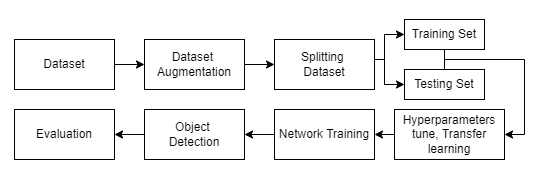
\includegraphics[scale=1]{40_Chapter_4/2.png}
    \caption{Working steps}
    \label{Working steps}
\end{figure}
The process of the entire project is depicted in Figure 2. We started by preprocessing the dataset. The dataset was separated into train and test sets after preprocessing. To develop the object detection model, DL techniques were used on the training set. The test set was then used to assess the models' performance.\\
\section{Dataset}
\subsection{Dataset Acquisition} Teeth photos with cavitation, micro-cavitation, and no cavitation were collected from several smartphones to form the tooth decay dataset. There are 233 pictures of teeth in varying stages of decay in the dataset. The dataset was manually annotated by human annotators and encoded in MS COCO format [11].
\subsection{Dataset Augmentation} We did data augmentation on the existing dataset to increase training and validation accuracy because the dataset only contains 233 photographs. Six augmentation techniques: vertical flip, horizontal flip, 90° rotation, horizontal-vertical flip, average blurring, and raise hue are utilized to turn the dataset into 2618 photos. 
\subsection{Removing Null Values} The dataset was uploaded to Roboflow [10] for image augmentation before training on YOLOv5s. Roboflow found 475 images with Null values after augmentation. Those were taken out of the dataset.
\subsection{Dataset Splitting} The dataset for YOLOv5s was divided into three parts: a training set with 86\% data (2266 images), a validation set with 9\% data (231 images), and a test set with 5\% data (images).

\section{Model Training} The dataset was trained in three YOLO object detection models.You Only Look Once is known by the acronym YOLO. This program identifies and finds different things in an image (in real-time). The class probabilities of the discovered photos are provided by the object identification process in YOLO, which is carried out as a regression problem. Convolutional neural networks (CNN) are used by the YOLO method to recognize items instantly. The approach just needs one forward propagation through a neural network to identify objects, as the name would imply. This indicates that a single algorithm run is used to do prediction throughout the full picture. Multiple class probabilities and bounding boxes are concurrently predicted using the CNN. YOLO algorithm works using the following three techniques:
\begin{enumerate}
    \item \textbf{Residual blocks: }The image is initially split into a number of grids. Each grid has a SxS dimension. There are several equal-sized grid cells. Every grid cell will be able to detect items that enter it. For instance, a grid cell will be in charge of detecting an item if its center appears within that cell.
    \item \textbf{Bounding box regression: }A bounding box is a highlighted outline of an item in a picture. The properties of each bounding box in the image are: Width, Height, Class, and Bounding box center. In order to determine the height, breadth, center, and class of an item, YOLO use a single bounding box regression.
    \item \textbf{Intersection over union (IOU): }Box overlapping is described by the object detection phenomena known as intersection over union (IOU). IOU is used by YOLO to create an output box that properly encircles the items. The predicted bounding boxes and their confidence scores are the responsibility of each grid cell. If the projected bounding box and the actual box match, the IOU is equal to 1. Bounding boxes that are not equivalent to the actual box are eliminated by this approach.
\end{enumerate}
\begin{figure}[H]
    \centering
    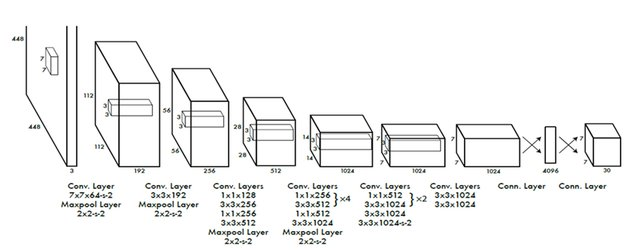
\includegraphics[scale=0.7]{40_Chapter_4/YOLO-architecture-YOLO-architecture-is-inspired-by-GooLeNet-model-for-image_W640.jpg}
    \caption{Yolo Architecture}
    \label{Architecture}
\end{figure}
Chosen models are: YOLOv4, YOLOv5, and YOLOv6. Model descriptions and how the dataset is trained on the model are described as follows: \\
\subsection{YOLOv4} The YOLOv4 algorithm is an enhanced version of the YOLOv3 method. It connects the YOLOv3 head with a CSP darknet-53 [12] classifier and spatial pyramid pooling. It benefits from excellent detection accuracy, precise bounding box positioning, and fast computations. YOLOv4 takes an image as input and compresses features using a backbone of convolutional neural networks. These backbones represent the network's endpoint in picture categorization, and they can be used to make predictions. YOLOv4 is pretrained on ImageNet classification [13]. We used the pretrained YOLOv4 weights and used it to train the model on our custom dataset via transfer learning [11].\\
\textbf{Activation Function: } Non-monotonic, smooth activation function Mish was chosen due to its minimal cost and qualities such as unbounded above and below, which boost its performance when compared to other often used functions. The Mish function has the following definition:
\begin{align*}
f(x)=x.tanh\left ( s\left ( x \right ) \right )\\
s(x)=ln\left (1+e^x \right )
\end{align*}
\myequations{Equation number \ref{eq:Eq1}}
S is a softmax activation function.\\
\subsection{YOLOv5:} YOLOv5 is available in four different models. Except for the model layer architecture and a few parameters, there are no significant differences between the versions [14]. We chose YOLOv5s and YOLOv5m as we had a limited dataset and trained the models from scratch to detect tooth decay. These two models were trained in two different settings to see which one performed better on our custom object detection. Stochastic Gradient Descent (SGD) optimization was used and the learning rate was 0.01.\\ 
\textbf{Activation Function: } YOLOv5 uses Leaky RelU activation function for hidden layers. The use of Leaky ReLU reduces the computation necessary to drive the neural network from growing exponentially. It has the following definition:\\
\begin{align*}
f\left ( y \right )= \left ( \alpha y \right ); if \left ( y< 0 \right )\\
f\left ( y \right )= \left (  y \right );if \left ( y> 0) \right ) 
\end{align*}
Sigmoid activation function that was used in the final detection layer. It transforms the input into a value between 0 and 1. The function is defined as follows: \\
\begin{align*}
Sigmoid s(x)=1/(1+e^-^x)
\end{align*}
\textbf{Loss Function: } Binary cross entropy loss function was used. Each of the projected probabilities is compared to the actual class output, which can be either 0 or 1. The score is then calculated, penalizing the probabilities based on their deviation from the predicted value.\\
\begin{align*}
 BCE= -\frac{1}{N}\sum_{i=1}^{N}\left ( y_{i} *y_{pred}+(1-y_{i})*log(1-y_{pred}))\right )
 \end{align*}
Where ypred is the ith scalar value in the model output and yi is the corresponding target value.
\subsection{YOLOv6} A team at the Chinese e-commerce platform business Meituan developed the object identification model known as YOLOv6. The term YOLOv6 is being used by the authors to save space even though the official name is MT-YOLOv6. They have essentially created the model on top of the YOLO (You Look Only Once) architecture and assert various advantages and new techniques over previous YOLO family models. PyTorch was used to create this framework. It adopted the decoupled head structure, taking into account the balance between the representation ability of the operators and the computing overhead on the hardware.It also adopted three strategies:\\
\begin{enumerate}
    \item \textbf{Anchor-free paradigm: } The anchor-free paradigm has gained popularity in recent years because of its excellent generalizability and straightforward code logic. The team discovered that the Anchor-free detector has a 51\% increase in speed when compared to previous techniques.
    \item \textbf{SimOTA Tag Assignment Policy: }The researchers employed the SimOTA method, which dynamically distributes positive samples to increase detection accuracy, to acquire high-quality positive samples.
    \item \textbf{SIoU bounding box regression loss: }To oversee the network's learning process, YOLOv6 uses the SIoU bounding box regression loss function. Through the addition of a vector angle between necessary regression, the SIoU loss function redefines the distance loss. As a consequence, the detection accuracy is enhanced as well as the regression accuracy.
\end{enumerate}
\section{Evaluation}
We should be prepared with several assessment metrics to examine the classification algorithm in the event of a classification problem. As follows:
\begin{enumerate}
    \item \textbf{Confusion Matrix:} The classification model's accuracy in classifying instances into distinct groups is summarized in a table called the confusion matrix. The model's anticipated label is on one axis of the confusion matrix, while the actual label is on the other. When comparing several models, we may use the confusion matrix to assess how well each one predicted true positives (TP) and true negatives (TN). We chose a model as our basic model if it accurately predicted TP and TN compared to other models.
\begin{figure}[H]
    \centering
    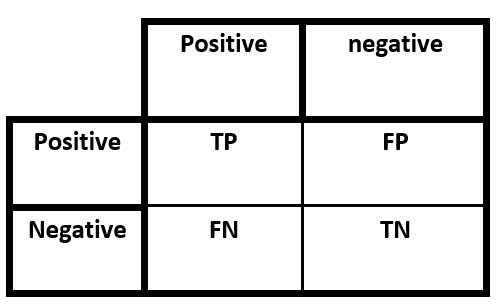
\includegraphics[scale=0.7]{40_Chapter_4/4.png}
    \caption{Confusion Matrix}
    \label{Confusion Matrix}
\end{figure}
TP = True Positive (The total number of images that are
correctly detected to be positive)\\
FP = False Positive (The total number of images that are
predicted to be positive but actually are negative)\\
TN = True Negative (The number of images that are
accurately predicted to be negative)\\
FN = False Negative (The number of images that are
incorrectly predicted to be negative)\\
    \item \textbf{Precision and Recall:} Precision and recall are two metrics used to evaluate classification and retrieval systems' performance. Precision is the percentage of relevant occurrences among all retrieved examples. Recall, also known as sensitivity, is the percentage of recovered instances among all appropriate models. In a perfect classifier, precision and recall are both one. 
\newline
\begin{align*}
Recall = \frac{TP}{TP+FP} 
\\
Precision = \frac{TP}{TP+FP}
\end{align*}
\newline
    \item \textbf{Accuracy:} It is calculated by dividing the total number of correctly categorized instances by the overall number of classified examples. When the importance of each class's prediction error is equal, this measure is crucial. Here, false positives should be addressed more than false negatives.
\newline
\begin{align*}
Accuracy = \frac{TP+tn}{TP+TN+FP+FN} 
\end{align*}
\newline
    \item \textbf{F1 score:} A weighted average of recall and accuracy is the F1 score. False positive and false negative results can occur in accuracy and recall, as is well known, thus both are taken into account. In most cases, the F1 score is more helpful than accuracy, particularly if your class is distributed unevenly. When false positives and false negatives cost about the same, accuracy performs best. It is preferable to include both Precision and Recall if the costs of false positives and false negatives are significantly different.
\newline
\begin{align*}
F1 Score = \frac{2*Recall*Precision}{Recall+Precision} 
\end{align*}
\newline
    \item \textbf{Learning Curve:} For algorithms that learn (optimize their internal parameters) gradually over time, like deep learning neural networks, learning curves are frequently employed in machine learning. If maximization is the metric used to measure learning, then higher scores (bigger numbers) signify more learning. Accuracy in categorisation might serve as an example. It is more typical to employ a score that minimizes, like loss or error, where better scores (lower numbers) imply greater learning and a value of 0.0 indicates that the training dataset was learnt properly with no errors. Additionally, a hold-out validation dataset that is separate from the training dataset can be used to test it. An assessment of the validation dataset provides insight into the model's "generalizability."
    \item \textbf{Learning Curve:} Mean Average Precision (mAP) is a popular metric for measuring how well object identification and segmentation systems perform. A statistic called Mean Average Precision (mAP) is used to assess object detection algorithms like Fast R-CNN, YOLO, Mask R-CNN, etc. Recall values between 0 and 1 are used to determine the average precision (AP) values. We need IOU, Precision, Recall, Precision Recall Curve, and AP in order to compute mAP [15][16]. The mAP was computed using the confidence threshold. 
    average precision $A P$
        $$
        \begin{aligned}
        &=\sum_{k=0}^{k=n-1}[\operatorname{Recall}(k)-\operatorname{Recall}(k+1) \\
        &* \text { Precision }(k)] \\
        &m A P=\frac{1}{n} \sum_{k=1}^{k=n} A P(k)
        \end{aligned}
        $$
        Where $\mathrm{AP}_{\mathrm{K}}=$ the $\mathrm{AP}$ of class $\mathrm{k}$
        
        $\mathrm{n}=$ number of classes
\end{enumerate}